\documentclass[12pt,aspectratio=43]{beamer}

% 自訂字體的封包
\usepackage{fontspec}

% 導入圖形與表格的封包
\usepackage{graphicx}
\graphicspath{{./20260114_Meeting}}

\usepackage{booktabs}

% 排列多個子圖形的封包
\usepackage{subfigure} 

 % 提供進階數學環境與公式排版
\usepackage{mathtools, amsmath, amsfonts, amsthm, latexsym}

%% 設定中文字體
\usepackage{xeCJK}
\setCJKmainfont[AutoFakeBold=3.5 , AutoFakeSlant=0.2]{標楷體}
\setmainfont{Times New Roman}
\XeTeXlinebreaklocale "zh"
\XeTeXlinebreakskip = 0pt plus 1pt

% 自訂字體顏色的封包
\usepackage{color} 

% 圖表自動編號的封包
\usepackage{caption}
% \usepackage{siunitx}

% 允許表格的一格能多列呈現的封包
\usepackage{multirow} 

% 可指定表格排版的封包
\usepackage{array}

% 翻轉表格的封包
\usepackage{lscape} 

% 序列標號
\usepackage{enumerate} 

%% 設定自動編號
\setbeamertemplate{caption}[numbered]

%% 自訂顏色
\definecolor{Myblue}{RGB}{57,108,144}
\definecolor{Default_Blue}{RGB}{52,51,171}

% (動畫)字會若隱若現的顯示
\beamersetuncovermixins{\opaqueness<1->{45}}{\opaqueness<1->{95}} 

% 設定中文的標籤
\renewcommand{\figurename}{圖} 
\renewcommand{\tablename}{表} 

% 排版形式 
\mode<presentation>{
\usetheme{Berlin}
% enumerate 及 item 的形狀
\setbeamertemplate{itemize items}[triangle]
% 調整外框形式的字體大小
\setbeamerfont{headline}{size=\scriptsize}
\setbeamerfont{footline}{size=\scriptsize}
% 取消右下方的跳轉工具列
\setbeamertemplate{navigation symbols}{} 
% 自定義2：清除外框下緣但僅出頁碼
\setbeamertemplate{footline}[page number] 
% 顏色主題
\usecolortheme{dove}
% 設定頁面邊界
\setbeamersize{text margin left=0.6cm, text margin right=0.6cm}
\special{papersize=\the\paperwidth,\the\paperheight}
\providecommand{\tabularnewline}{\\}
}

\title{Meeting 0114}
\author{黃丞暘}
\institute{國立東華大學應數統計所}
\date{January 14, 2026}

\begin{document}

% 封面
\begin{frame}
  \titlepage
\end{frame}

% 目錄
\begin{frame}{\textbf{Index}}
  \tableofcontents
\end{frame}

% DISCUSSION 
\section{01/07 Discussion}

\begin{frame}{\textbf{01/07 Discussion}}
\linespread{1.5}
Semiconductor Manufacturing Process

  \begin{itemize}
    \item \textbf{原始空間下的資料生成（避免外插）}
    \begin{enumerate}[]
      \item 低維（或降維後）平面上找點做資料就像外插法，放到原始（p維）空間可能落在資料範圍外或出現機率極低
    \end{enumerate}
    \item \textbf{隨機擾動與 local 擬合度（$R^2$）}
    \begin{enumerate}[]
      \item 樣本數小：擾動多集中在點附近，相當於較小範圍做local近似，linear surrogate 的 $R^2$ 偏高
      \item 樣本數大：同個 $\sigma$下會抽到更遠的尾端點，相當於較大範圍做local 近似；對非線性時，linear surrogate 的 $R^2$ 下降且分散
    \end{enumerate}
  \end{itemize}
\end{frame}


% TO DO
\section{01/07 Todo}

\begin{frame}{\textbf{01/07 Todo}}
\linespread{1.5}
  \begin{itemize}
    \item \textbf{Separate and fit black-box function}
    \begin{enumerate}[]
      \item 將資料切分：$\mathcal{D}_c=\{(x_i, y_i):c_i=c\}$，其中$c \in \{1,...,K\}$，
      對每個 cluster 獨立訓練 black-box $\hat{f}_c:x\longmapsto\hat{p}_c(x)$
    \end{enumerate}
  \end{itemize}

  \begin{itemize}
    \item \textbf{Re-build $\hat f$ through local linear regression}
    \begin{enumerate}[]
      \item 於各 cluster 內挑選滿足 $\hat p_c(x_0)\approx 0.5/1$ 的樣本點集合，取平均$\bar x_0$，並以其為中心生成 
      lattice cube 擾動點 $\{x_{\ell}\}$
      \item 代入 black-box 取得局部輸出：$y_{\ell}=\hat p_c(x_{\ell})$
      \item 以線性迴歸 fit local surrogate $\hat g(\cdot;\bar x_0)$，得到局部線性近似 $\hat f(x)\approx \hat g(x;\bar x_0)$
    \end{enumerate}
  \end{itemize}
\end{frame}

% 結果
\section{Results - What I did this time}

\begin{frame}{\textbf{Results I}　{SMOTE + PCA + KMeans}}
\linespread{0.9}

\begin{center}
  \begin{minipage}{0.45\linewidth}
    \centering
    
\includegraphics[width=\linewidth]{pca.png}
  \end{minipage}
  \hspace{0.3em}
  \begin{minipage}{0.45\linewidth}
    \centering
    
\includegraphics[width=\linewidth]{pca2.png}
  \end{minipage}
\end{center}

\small{$$
\begin{array}{c|cc}
\text{cluster} & 0 & 1 \\
\hline
y=0 & 743 & 687 \\
y=1 & 205 & 510 \\
\end{array}
$$}

\end{frame}

\begin{frame}{Separate and build local surrogate models}
\linespread{1.2}
  \begin{itemize}
    \item 在各群內分別訓練分類 black-box $\hat f_c$，並以 $\hat p_c(x)=\Pr(\hat y=1\mid x)$ 表示其輸出機率
    \item 在群 $c$ 內，挑選滿足 $\hat p_c(x_0)\approx 0.5/1$(fail) 的代表點，
    並在各群內以 K-fold CV 取得 out-of-fold $\hat p$，於每折 test 取 $\hat p\approx 0.5/1$(fail) 的 $x_0^{(fold)}$，再將其平均得中心點 $\bar x_0$
    \item 生成局部格點（lattice cube）擾動樣本：在標準化空間以步長 $\delta$、半徑層數 $k$ 於 $\bar x_0$ 周圍取樣，得到 $\{x_{\ell}\}$
    \item 代入對應的 cluster black-box：$y_{\ell}=\hat p_c(x_{\ell})$
    \item 以 $\{(x_{\ell},y_{\ell})\}$ fit local surrogate $\hat g(\cdot;\bar x_0)$，
          使得在 $\bar x_0$ 附近內 $\hat p_c(x)\approx \hat g(x;\bar x_0)$
  \end{itemize}
\end{frame}

\begin{frame}{\textbf{Results II}　{f\_logistic\& g\_linear}}
\begin{center}
  \begin{minipage}{0.7\linewidth}
    \centering
    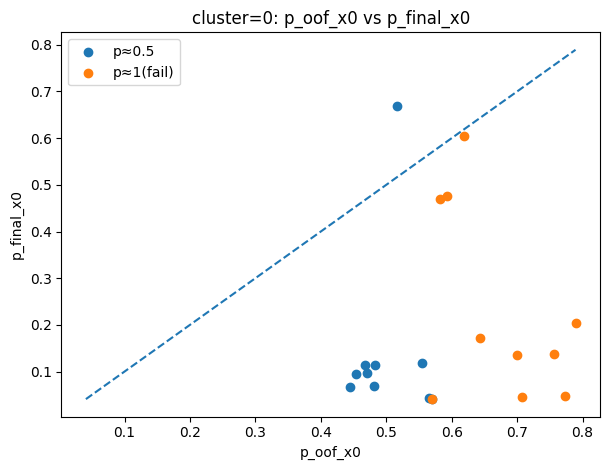
\includegraphics[width=\linewidth]{fig_oof_vs_final_cluster0.png} 
  \end{minipage}
\end{center}
\end{frame}

\begin{frame}{\textbf{Results II}　{f\_logistic\& g\_linear}}
\begin{center}
  \begin{minipage}{.7\linewidth}
    \centering
    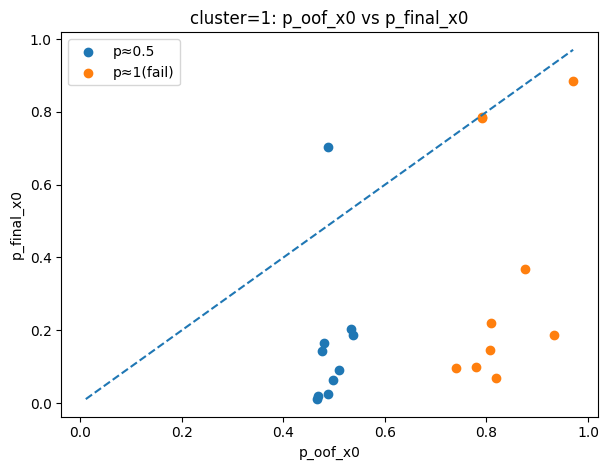
\includegraphics[width=\linewidth]{fig_oof_vs_final_cluster1.png}
  \end{minipage}
\end{center}
\end{frame}

\begin{frame}{\textbf{Results II}　{f\_logistic\& g\_linear}}
\begin{center}
  \begin{minipage}{.7\linewidth}
    \centering
    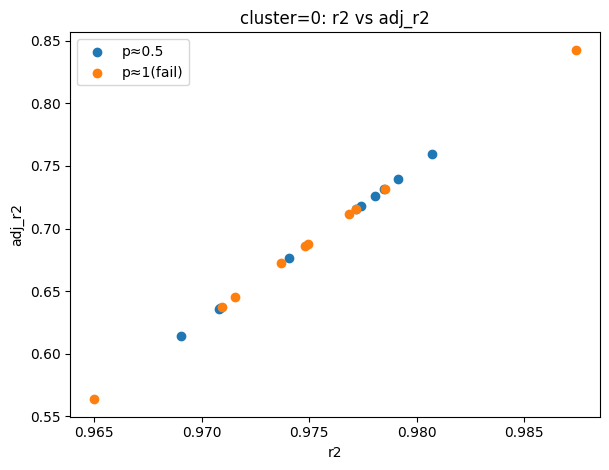
\includegraphics[width=\linewidth]{r2 vs adj_r2 _cluster0.png}
  \end{minipage}
\end{center}
\end{frame}

\begin{frame}{\textbf{Results II}　{f\_logistic\& g\_linear}}
\begin{center}
  \begin{minipage}{.7\linewidth}
    \centering
    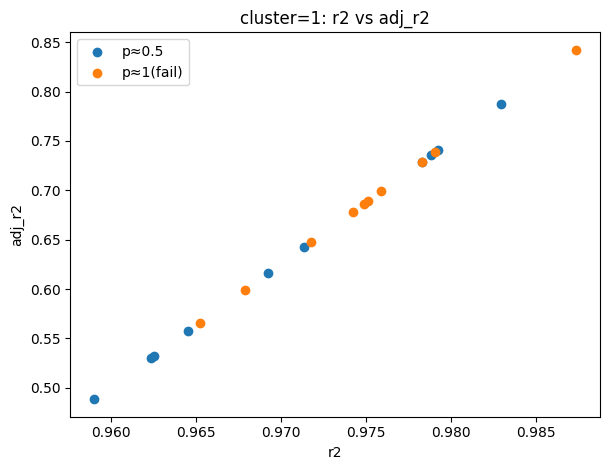
\includegraphics[width=\linewidth]{r2 vs adj_r2 _cluster1.png}
  \end{minipage}
\end{center}
\end{frame}

\begin{frame}{\textbf{Results II}　{f\_logistic\& g\_linear}}

  $$
  \begin{array}{c|rcccccc}
  x0\_index & p\_\text{oof} & p\_\text{final} & r2 & \text{adj\_}r2 & mse \\
  \hline
  1361 & 0.516 & 0.669 & 0.971 & 0.636  & 0.000 \\
  \phantom{0}995 & 0.482 & 0.115 & 0.971 & 0.636  & 0.000 \\
  1108 & 0.481 & 0.070 & 0.978 & 0.726  & 0.000 \\
  1227 & 0.471 & 0.096 & 0.979 & 0.740  & 0.000 \\
  \phantom{0}507 & 0.468 & 0.114 & 0.974 & 0.676  & 0.000 \\
  \end{array}
  $$

  $$
  \begin{array}{c|rccc}
  \text{term} & \text{coef} & \text{p-value} & \text{95\% CI}\\
  \hline
  \text{const} & -0.2039 & 0.000 & [-0.204,\,-0.204]\\
  x_1 & -0.0087 & 0.000 & [-0.009,\,-0.009]\\
  x_2 & -0.0214 & 0.000 & [-0.021,\,-0.021]\\
  x_3 & -0.0038 & 0.000 & [-0.004,\,-0.004]\\
  x_4 & -0.0215 & 0.000 & [-0.022,\,-0.022]\\
  \end{array}
  $$
\end{frame}

% --- 結束 ---
\section*{結束}

\begin{frame}[plain] % 產生無外框的頁面
	\begin{center}
		{\Huge The End}
		\bigskip\bigskip 

		{\LARGE Questions  \&  Comments}
	\end{center}
\end{frame}
\end{document}ㄒ
